\documentclass[11pt]{article}

    \usepackage[breakable]{tcolorbox}
    \usepackage{parskip} % Stop auto-indenting (to mimic markdown behaviour)
    

    % Basic figure setup, for now with no caption control since it's done
    % automatically by Pandoc (which extracts ![](path) syntax from Markdown).
    \usepackage{graphicx}
    % Maintain compatibility with old templates. Remove in nbconvert 6.0
    \let\Oldincludegraphics\includegraphics
    % Ensure that by default, figures have no caption (until we provide a
    % proper Figure object with a Caption API and a way to capture that
    % in the conversion process - todo).
    \usepackage{caption}
    \DeclareCaptionFormat{nocaption}{}
    \captionsetup{format=nocaption,aboveskip=0pt,belowskip=0pt}

    \usepackage{float}
    \floatplacement{figure}{H} % forces figures to be placed at the correct location
    \usepackage{xcolor} % Allow colors to be defined
    \usepackage{enumerate} % Needed for markdown enumerations to work
    \usepackage{geometry} % Used to adjust the document margins
    \usepackage{amsmath} % Equations
    \usepackage{amssymb} % Equations
    \usepackage{textcomp} % defines textquotesingle
    % Hack from http://tex.stackexchange.com/a/47451/13684:
    \AtBeginDocument{%
        \def\PYZsq{\textquotesingle}% Upright quotes in Pygmentized code
    }
    \usepackage{upquote} % Upright quotes for verbatim code
    \usepackage{eurosym} % defines \euro

    \usepackage{iftex}
    \ifPDFTeX
        \usepackage[T1]{fontenc}
        \IfFileExists{alphabeta.sty}{
              \usepackage{alphabeta}
          }{
              \usepackage[mathletters]{ucs}
              \usepackage[utf8x]{inputenc}
          }
    \else
        \usepackage{fontspec}
        \usepackage{unicode-math}
    \fi

    \usepackage{fancyvrb} % verbatim replacement that allows latex
    \usepackage{grffile} % extends the file name processing of package graphics
                         % to support a larger range
    \makeatletter % fix for old versions of grffile with XeLaTeX
    \@ifpackagelater{grffile}{2019/11/01}
    {
      % Do nothing on new versions
    }
    {
      \def\Gread@@xetex#1{%
        \IfFileExists{"\Gin@base".bb}%
        {\Gread@eps{\Gin@base.bb}}%
        {\Gread@@xetex@aux#1}%
      }
    }
    \makeatother
    \usepackage[Export]{adjustbox} % Used to constrain images to a maximum size
    \adjustboxset{max size={0.9\linewidth}{0.9\paperheight}}

    % The hyperref package gives us a pdf with properly built
    % internal navigation ('pdf bookmarks' for the table of contents,
    % internal cross-reference links, web links for URLs, etc.)
    \usepackage{hyperref}
    % The default LaTeX title has an obnoxious amount of whitespace. By default,
    % titling removes some of it. It also provides customization options.
    \usepackage{titling}
    \usepackage{longtable} % longtable support required by pandoc >1.10
    \usepackage{booktabs}  % table support for pandoc > 1.12.2
    \usepackage{array}     % table support for pandoc >= 2.11.3
    \usepackage{calc}      % table minipage width calculation for pandoc >= 2.11.1
    \usepackage[inline]{enumitem} % IRkernel/repr support (it uses the enumerate* environment)
    \usepackage[normalem]{ulem} % ulem is needed to support strikethroughs (\sout)
                                % normalem makes italics be italics, not underlines
    \usepackage{soul}      % strikethrough (\st) support for pandoc >= 3.0.0
    \usepackage{mathrsfs}
    

    
    % Colors for the hyperref package
    \definecolor{urlcolor}{rgb}{0,.145,.698}
    \definecolor{linkcolor}{rgb}{.71,0.21,0.01}
    \definecolor{citecolor}{rgb}{.12,.54,.11}

    % ANSI colors
    \definecolor{ansi-black}{HTML}{3E424D}
    \definecolor{ansi-black-intense}{HTML}{282C36}
    \definecolor{ansi-red}{HTML}{E75C58}
    \definecolor{ansi-red-intense}{HTML}{B22B31}
    \definecolor{ansi-green}{HTML}{00A250}
    \definecolor{ansi-green-intense}{HTML}{007427}
    \definecolor{ansi-yellow}{HTML}{DDB62B}
    \definecolor{ansi-yellow-intense}{HTML}{B27D12}
    \definecolor{ansi-blue}{HTML}{208FFB}
    \definecolor{ansi-blue-intense}{HTML}{0065CA}
    \definecolor{ansi-magenta}{HTML}{D160C4}
    \definecolor{ansi-magenta-intense}{HTML}{A03196}
    \definecolor{ansi-cyan}{HTML}{60C6C8}
    \definecolor{ansi-cyan-intense}{HTML}{258F8F}
    \definecolor{ansi-white}{HTML}{C5C1B4}
    \definecolor{ansi-white-intense}{HTML}{A1A6B2}
    \definecolor{ansi-default-inverse-fg}{HTML}{FFFFFF}
    \definecolor{ansi-default-inverse-bg}{HTML}{000000}

    % common color for the border for error outputs.
    \definecolor{outerrorbackground}{HTML}{FFDFDF}

    % commands and environments needed by pandoc snippets
    % extracted from the output of `pandoc -s`
    \providecommand{\tightlist}{%
      \setlength{\itemsep}{0pt}\setlength{\parskip}{0pt}}
    \DefineVerbatimEnvironment{Highlighting}{Verbatim}{commandchars=\\\{\}}
    % Add ',fontsize=\small' for more characters per line
    \newenvironment{Shaded}{}{}
    \newcommand{\KeywordTok}[1]{\textcolor[rgb]{0.00,0.44,0.13}{\textbf{{#1}}}}
    \newcommand{\DataTypeTok}[1]{\textcolor[rgb]{0.56,0.13,0.00}{{#1}}}
    \newcommand{\DecValTok}[1]{\textcolor[rgb]{0.25,0.63,0.44}{{#1}}}
    \newcommand{\BaseNTok}[1]{\textcolor[rgb]{0.25,0.63,0.44}{{#1}}}
    \newcommand{\FloatTok}[1]{\textcolor[rgb]{0.25,0.63,0.44}{{#1}}}
    \newcommand{\CharTok}[1]{\textcolor[rgb]{0.25,0.44,0.63}{{#1}}}
    \newcommand{\StringTok}[1]{\textcolor[rgb]{0.25,0.44,0.63}{{#1}}}
    \newcommand{\CommentTok}[1]{\textcolor[rgb]{0.38,0.63,0.69}{\textit{{#1}}}}
    \newcommand{\OtherTok}[1]{\textcolor[rgb]{0.00,0.44,0.13}{{#1}}}
    \newcommand{\AlertTok}[1]{\textcolor[rgb]{1.00,0.00,0.00}{\textbf{{#1}}}}
    \newcommand{\FunctionTok}[1]{\textcolor[rgb]{0.02,0.16,0.49}{{#1}}}
    \newcommand{\RegionMarkerTok}[1]{{#1}}
    \newcommand{\ErrorTok}[1]{\textcolor[rgb]{1.00,0.00,0.00}{\textbf{{#1}}}}
    \newcommand{\NormalTok}[1]{{#1}}

    % Additional commands for more recent versions of Pandoc
    \newcommand{\ConstantTok}[1]{\textcolor[rgb]{0.53,0.00,0.00}{{#1}}}
    \newcommand{\SpecialCharTok}[1]{\textcolor[rgb]{0.25,0.44,0.63}{{#1}}}
    \newcommand{\VerbatimStringTok}[1]{\textcolor[rgb]{0.25,0.44,0.63}{{#1}}}
    \newcommand{\SpecialStringTok}[1]{\textcolor[rgb]{0.73,0.40,0.53}{{#1}}}
    \newcommand{\ImportTok}[1]{{#1}}
    \newcommand{\DocumentationTok}[1]{\textcolor[rgb]{0.73,0.13,0.13}{\textit{{#1}}}}
    \newcommand{\AnnotationTok}[1]{\textcolor[rgb]{0.38,0.63,0.69}{\textbf{\textit{{#1}}}}}
    \newcommand{\CommentVarTok}[1]{\textcolor[rgb]{0.38,0.63,0.69}{\textbf{\textit{{#1}}}}}
    \newcommand{\VariableTok}[1]{\textcolor[rgb]{0.10,0.09,0.49}{{#1}}}
    \newcommand{\ControlFlowTok}[1]{\textcolor[rgb]{0.00,0.44,0.13}{\textbf{{#1}}}}
    \newcommand{\OperatorTok}[1]{\textcolor[rgb]{0.40,0.40,0.40}{{#1}}}
    \newcommand{\BuiltInTok}[1]{{#1}}
    \newcommand{\ExtensionTok}[1]{{#1}}
    \newcommand{\PreprocessorTok}[1]{\textcolor[rgb]{0.74,0.48,0.00}{{#1}}}
    \newcommand{\AttributeTok}[1]{\textcolor[rgb]{0.49,0.56,0.16}{{#1}}}
    \newcommand{\InformationTok}[1]{\textcolor[rgb]{0.38,0.63,0.69}{\textbf{\textit{{#1}}}}}
    \newcommand{\WarningTok}[1]{\textcolor[rgb]{0.38,0.63,0.69}{\textbf{\textit{{#1}}}}}


    % Define a nice break command that doesn't care if a line doesn't already
    % exist.
    \def\br{\hspace*{\fill} \\* }
    % Math Jax compatibility definitions
    \def\gt{>}
    \def\lt{<}
    \let\Oldtex\TeX
    \let\Oldlatex\LaTeX
    \renewcommand{\TeX}{\textrm{\Oldtex}}
    \renewcommand{\LaTeX}{\textrm{\Oldlatex}}
    % Document parameters
    % Document title
    \title{lab9}
    
    
    
    
    
    
    
% Pygments definitions
\makeatletter
\def\PY@reset{\let\PY@it=\relax \let\PY@bf=\relax%
    \let\PY@ul=\relax \let\PY@tc=\relax%
    \let\PY@bc=\relax \let\PY@ff=\relax}
\def\PY@tok#1{\csname PY@tok@#1\endcsname}
\def\PY@toks#1+{\ifx\relax#1\empty\else%
    \PY@tok{#1}\expandafter\PY@toks\fi}
\def\PY@do#1{\PY@bc{\PY@tc{\PY@ul{%
    \PY@it{\PY@bf{\PY@ff{#1}}}}}}}
\def\PY#1#2{\PY@reset\PY@toks#1+\relax+\PY@do{#2}}

\@namedef{PY@tok@w}{\def\PY@tc##1{\textcolor[rgb]{0.73,0.73,0.73}{##1}}}
\@namedef{PY@tok@c}{\let\PY@it=\textit\def\PY@tc##1{\textcolor[rgb]{0.24,0.48,0.48}{##1}}}
\@namedef{PY@tok@cp}{\def\PY@tc##1{\textcolor[rgb]{0.61,0.40,0.00}{##1}}}
\@namedef{PY@tok@k}{\let\PY@bf=\textbf\def\PY@tc##1{\textcolor[rgb]{0.00,0.50,0.00}{##1}}}
\@namedef{PY@tok@kp}{\def\PY@tc##1{\textcolor[rgb]{0.00,0.50,0.00}{##1}}}
\@namedef{PY@tok@kt}{\def\PY@tc##1{\textcolor[rgb]{0.69,0.00,0.25}{##1}}}
\@namedef{PY@tok@o}{\def\PY@tc##1{\textcolor[rgb]{0.40,0.40,0.40}{##1}}}
\@namedef{PY@tok@ow}{\let\PY@bf=\textbf\def\PY@tc##1{\textcolor[rgb]{0.67,0.13,1.00}{##1}}}
\@namedef{PY@tok@nb}{\def\PY@tc##1{\textcolor[rgb]{0.00,0.50,0.00}{##1}}}
\@namedef{PY@tok@nf}{\def\PY@tc##1{\textcolor[rgb]{0.00,0.00,1.00}{##1}}}
\@namedef{PY@tok@nc}{\let\PY@bf=\textbf\def\PY@tc##1{\textcolor[rgb]{0.00,0.00,1.00}{##1}}}
\@namedef{PY@tok@nn}{\let\PY@bf=\textbf\def\PY@tc##1{\textcolor[rgb]{0.00,0.00,1.00}{##1}}}
\@namedef{PY@tok@ne}{\let\PY@bf=\textbf\def\PY@tc##1{\textcolor[rgb]{0.80,0.25,0.22}{##1}}}
\@namedef{PY@tok@nv}{\def\PY@tc##1{\textcolor[rgb]{0.10,0.09,0.49}{##1}}}
\@namedef{PY@tok@no}{\def\PY@tc##1{\textcolor[rgb]{0.53,0.00,0.00}{##1}}}
\@namedef{PY@tok@nl}{\def\PY@tc##1{\textcolor[rgb]{0.46,0.46,0.00}{##1}}}
\@namedef{PY@tok@ni}{\let\PY@bf=\textbf\def\PY@tc##1{\textcolor[rgb]{0.44,0.44,0.44}{##1}}}
\@namedef{PY@tok@na}{\def\PY@tc##1{\textcolor[rgb]{0.41,0.47,0.13}{##1}}}
\@namedef{PY@tok@nt}{\let\PY@bf=\textbf\def\PY@tc##1{\textcolor[rgb]{0.00,0.50,0.00}{##1}}}
\@namedef{PY@tok@nd}{\def\PY@tc##1{\textcolor[rgb]{0.67,0.13,1.00}{##1}}}
\@namedef{PY@tok@s}{\def\PY@tc##1{\textcolor[rgb]{0.73,0.13,0.13}{##1}}}
\@namedef{PY@tok@sd}{\let\PY@it=\textit\def\PY@tc##1{\textcolor[rgb]{0.73,0.13,0.13}{##1}}}
\@namedef{PY@tok@si}{\let\PY@bf=\textbf\def\PY@tc##1{\textcolor[rgb]{0.64,0.35,0.47}{##1}}}
\@namedef{PY@tok@se}{\let\PY@bf=\textbf\def\PY@tc##1{\textcolor[rgb]{0.67,0.36,0.12}{##1}}}
\@namedef{PY@tok@sr}{\def\PY@tc##1{\textcolor[rgb]{0.64,0.35,0.47}{##1}}}
\@namedef{PY@tok@ss}{\def\PY@tc##1{\textcolor[rgb]{0.10,0.09,0.49}{##1}}}
\@namedef{PY@tok@sx}{\def\PY@tc##1{\textcolor[rgb]{0.00,0.50,0.00}{##1}}}
\@namedef{PY@tok@m}{\def\PY@tc##1{\textcolor[rgb]{0.40,0.40,0.40}{##1}}}
\@namedef{PY@tok@gh}{\let\PY@bf=\textbf\def\PY@tc##1{\textcolor[rgb]{0.00,0.00,0.50}{##1}}}
\@namedef{PY@tok@gu}{\let\PY@bf=\textbf\def\PY@tc##1{\textcolor[rgb]{0.50,0.00,0.50}{##1}}}
\@namedef{PY@tok@gd}{\def\PY@tc##1{\textcolor[rgb]{0.63,0.00,0.00}{##1}}}
\@namedef{PY@tok@gi}{\def\PY@tc##1{\textcolor[rgb]{0.00,0.52,0.00}{##1}}}
\@namedef{PY@tok@gr}{\def\PY@tc##1{\textcolor[rgb]{0.89,0.00,0.00}{##1}}}
\@namedef{PY@tok@ge}{\let\PY@it=\textit}
\@namedef{PY@tok@gs}{\let\PY@bf=\textbf}
\@namedef{PY@tok@ges}{\let\PY@bf=\textbf\let\PY@it=\textit}
\@namedef{PY@tok@gp}{\let\PY@bf=\textbf\def\PY@tc##1{\textcolor[rgb]{0.00,0.00,0.50}{##1}}}
\@namedef{PY@tok@go}{\def\PY@tc##1{\textcolor[rgb]{0.44,0.44,0.44}{##1}}}
\@namedef{PY@tok@gt}{\def\PY@tc##1{\textcolor[rgb]{0.00,0.27,0.87}{##1}}}
\@namedef{PY@tok@err}{\def\PY@bc##1{{\setlength{\fboxsep}{\string -\fboxrule}\fcolorbox[rgb]{1.00,0.00,0.00}{1,1,1}{\strut ##1}}}}
\@namedef{PY@tok@kc}{\let\PY@bf=\textbf\def\PY@tc##1{\textcolor[rgb]{0.00,0.50,0.00}{##1}}}
\@namedef{PY@tok@kd}{\let\PY@bf=\textbf\def\PY@tc##1{\textcolor[rgb]{0.00,0.50,0.00}{##1}}}
\@namedef{PY@tok@kn}{\let\PY@bf=\textbf\def\PY@tc##1{\textcolor[rgb]{0.00,0.50,0.00}{##1}}}
\@namedef{PY@tok@kr}{\let\PY@bf=\textbf\def\PY@tc##1{\textcolor[rgb]{0.00,0.50,0.00}{##1}}}
\@namedef{PY@tok@bp}{\def\PY@tc##1{\textcolor[rgb]{0.00,0.50,0.00}{##1}}}
\@namedef{PY@tok@fm}{\def\PY@tc##1{\textcolor[rgb]{0.00,0.00,1.00}{##1}}}
\@namedef{PY@tok@vc}{\def\PY@tc##1{\textcolor[rgb]{0.10,0.09,0.49}{##1}}}
\@namedef{PY@tok@vg}{\def\PY@tc##1{\textcolor[rgb]{0.10,0.09,0.49}{##1}}}
\@namedef{PY@tok@vi}{\def\PY@tc##1{\textcolor[rgb]{0.10,0.09,0.49}{##1}}}
\@namedef{PY@tok@vm}{\def\PY@tc##1{\textcolor[rgb]{0.10,0.09,0.49}{##1}}}
\@namedef{PY@tok@sa}{\def\PY@tc##1{\textcolor[rgb]{0.73,0.13,0.13}{##1}}}
\@namedef{PY@tok@sb}{\def\PY@tc##1{\textcolor[rgb]{0.73,0.13,0.13}{##1}}}
\@namedef{PY@tok@sc}{\def\PY@tc##1{\textcolor[rgb]{0.73,0.13,0.13}{##1}}}
\@namedef{PY@tok@dl}{\def\PY@tc##1{\textcolor[rgb]{0.73,0.13,0.13}{##1}}}
\@namedef{PY@tok@s2}{\def\PY@tc##1{\textcolor[rgb]{0.73,0.13,0.13}{##1}}}
\@namedef{PY@tok@sh}{\def\PY@tc##1{\textcolor[rgb]{0.73,0.13,0.13}{##1}}}
\@namedef{PY@tok@s1}{\def\PY@tc##1{\textcolor[rgb]{0.73,0.13,0.13}{##1}}}
\@namedef{PY@tok@mb}{\def\PY@tc##1{\textcolor[rgb]{0.40,0.40,0.40}{##1}}}
\@namedef{PY@tok@mf}{\def\PY@tc##1{\textcolor[rgb]{0.40,0.40,0.40}{##1}}}
\@namedef{PY@tok@mh}{\def\PY@tc##1{\textcolor[rgb]{0.40,0.40,0.40}{##1}}}
\@namedef{PY@tok@mi}{\def\PY@tc##1{\textcolor[rgb]{0.40,0.40,0.40}{##1}}}
\@namedef{PY@tok@il}{\def\PY@tc##1{\textcolor[rgb]{0.40,0.40,0.40}{##1}}}
\@namedef{PY@tok@mo}{\def\PY@tc##1{\textcolor[rgb]{0.40,0.40,0.40}{##1}}}
\@namedef{PY@tok@ch}{\let\PY@it=\textit\def\PY@tc##1{\textcolor[rgb]{0.24,0.48,0.48}{##1}}}
\@namedef{PY@tok@cm}{\let\PY@it=\textit\def\PY@tc##1{\textcolor[rgb]{0.24,0.48,0.48}{##1}}}
\@namedef{PY@tok@cpf}{\let\PY@it=\textit\def\PY@tc##1{\textcolor[rgb]{0.24,0.48,0.48}{##1}}}
\@namedef{PY@tok@c1}{\let\PY@it=\textit\def\PY@tc##1{\textcolor[rgb]{0.24,0.48,0.48}{##1}}}
\@namedef{PY@tok@cs}{\let\PY@it=\textit\def\PY@tc##1{\textcolor[rgb]{0.24,0.48,0.48}{##1}}}

\def\PYZbs{\char`\\}
\def\PYZus{\char`\_}
\def\PYZob{\char`\{}
\def\PYZcb{\char`\}}
\def\PYZca{\char`\^}
\def\PYZam{\char`\&}
\def\PYZlt{\char`\<}
\def\PYZgt{\char`\>}
\def\PYZsh{\char`\#}
\def\PYZpc{\char`\%}
\def\PYZdl{\char`\$}
\def\PYZhy{\char`\-}
\def\PYZsq{\char`\'}
\def\PYZdq{\char`\"}
\def\PYZti{\char`\~}
% for compatibility with earlier versions
\def\PYZat{@}
\def\PYZlb{[}
\def\PYZrb{]}
\makeatother


    % For linebreaks inside Verbatim environment from package fancyvrb.
    \makeatletter
        \newbox\Wrappedcontinuationbox
        \newbox\Wrappedvisiblespacebox
        \newcommand*\Wrappedvisiblespace {\textcolor{red}{\textvisiblespace}}
        \newcommand*\Wrappedcontinuationsymbol {\textcolor{red}{\llap{\tiny$\m@th\hookrightarrow$}}}
        \newcommand*\Wrappedcontinuationindent {3ex }
        \newcommand*\Wrappedafterbreak {\kern\Wrappedcontinuationindent\copy\Wrappedcontinuationbox}
        % Take advantage of the already applied Pygments mark-up to insert
        % potential linebreaks for TeX processing.
        %        {, <, #, %, $, ' and ": go to next line.
        %        _, }, ^, &, >, - and ~: stay at end of broken line.
        % Use of \textquotesingle for straight quote.
        \newcommand*\Wrappedbreaksatspecials {%
            \def\PYGZus{\discretionary{\char`\_}{\Wrappedafterbreak}{\char`\_}}%
            \def\PYGZob{\discretionary{}{\Wrappedafterbreak\char`\{}{\char`\{}}%
            \def\PYGZcb{\discretionary{\char`\}}{\Wrappedafterbreak}{\char`\}}}%
            \def\PYGZca{\discretionary{\char`\^}{\Wrappedafterbreak}{\char`\^}}%
            \def\PYGZam{\discretionary{\char`\&}{\Wrappedafterbreak}{\char`\&}}%
            \def\PYGZlt{\discretionary{}{\Wrappedafterbreak\char`\<}{\char`\<}}%
            \def\PYGZgt{\discretionary{\char`\>}{\Wrappedafterbreak}{\char`\>}}%
            \def\PYGZsh{\discretionary{}{\Wrappedafterbreak\char`\#}{\char`\#}}%
            \def\PYGZpc{\discretionary{}{\Wrappedafterbreak\char`\%}{\char`\%}}%
            \def\PYGZdl{\discretionary{}{\Wrappedafterbreak\char`\$}{\char`\$}}%
            \def\PYGZhy{\discretionary{\char`\-}{\Wrappedafterbreak}{\char`\-}}%
            \def\PYGZsq{\discretionary{}{\Wrappedafterbreak\textquotesingle}{\textquotesingle}}%
            \def\PYGZdq{\discretionary{}{\Wrappedafterbreak\char`\"}{\char`\"}}%
            \def\PYGZti{\discretionary{\char`\~}{\Wrappedafterbreak}{\char`\~}}%
        }
        % Some characters . , ; ? ! / are not pygmentized.
        % This macro makes them "active" and they will insert potential linebreaks
        \newcommand*\Wrappedbreaksatpunct {%
            \lccode`\~`\.\lowercase{\def~}{\discretionary{\hbox{\char`\.}}{\Wrappedafterbreak}{\hbox{\char`\.}}}%
            \lccode`\~`\,\lowercase{\def~}{\discretionary{\hbox{\char`\,}}{\Wrappedafterbreak}{\hbox{\char`\,}}}%
            \lccode`\~`\;\lowercase{\def~}{\discretionary{\hbox{\char`\;}}{\Wrappedafterbreak}{\hbox{\char`\;}}}%
            \lccode`\~`\:\lowercase{\def~}{\discretionary{\hbox{\char`\:}}{\Wrappedafterbreak}{\hbox{\char`\:}}}%
            \lccode`\~`\?\lowercase{\def~}{\discretionary{\hbox{\char`\?}}{\Wrappedafterbreak}{\hbox{\char`\?}}}%
            \lccode`\~`\!\lowercase{\def~}{\discretionary{\hbox{\char`\!}}{\Wrappedafterbreak}{\hbox{\char`\!}}}%
            \lccode`\~`\/\lowercase{\def~}{\discretionary{\hbox{\char`\/}}{\Wrappedafterbreak}{\hbox{\char`\/}}}%
            \catcode`\.\active
            \catcode`\,\active
            \catcode`\;\active
            \catcode`\:\active
            \catcode`\?\active
            \catcode`\!\active
            \catcode`\/\active
            \lccode`\~`\~
        }
    \makeatother

    \let\OriginalVerbatim=\Verbatim
    \makeatletter
    \renewcommand{\Verbatim}[1][1]{%
        %\parskip\z@skip
        \sbox\Wrappedcontinuationbox {\Wrappedcontinuationsymbol}%
        \sbox\Wrappedvisiblespacebox {\FV@SetupFont\Wrappedvisiblespace}%
        \def\FancyVerbFormatLine ##1{\hsize\linewidth
            \vtop{\raggedright\hyphenpenalty\z@\exhyphenpenalty\z@
                \doublehyphendemerits\z@\finalhyphendemerits\z@
                \strut ##1\strut}%
        }%
        % If the linebreak is at a space, the latter will be displayed as visible
        % space at end of first line, and a continuation symbol starts next line.
        % Stretch/shrink are however usually zero for typewriter font.
        \def\FV@Space {%
            \nobreak\hskip\z@ plus\fontdimen3\font minus\fontdimen4\font
            \discretionary{\copy\Wrappedvisiblespacebox}{\Wrappedafterbreak}
            {\kern\fontdimen2\font}%
        }%

        % Allow breaks at special characters using \PYG... macros.
        \Wrappedbreaksatspecials
        % Breaks at punctuation characters . , ; ? ! and / need catcode=\active
        \OriginalVerbatim[#1,codes*=\Wrappedbreaksatpunct]%
    }
    \makeatother

    % Exact colors from NB
    \definecolor{incolor}{HTML}{303F9F}
    \definecolor{outcolor}{HTML}{D84315}
    \definecolor{cellborder}{HTML}{CFCFCF}
    \definecolor{cellbackground}{HTML}{F7F7F7}

    % prompt
    \makeatletter
    \newcommand{\boxspacing}{\kern\kvtcb@left@rule\kern\kvtcb@boxsep}
    \makeatother
    \newcommand{\prompt}[4]{
        {\ttfamily\llap{{\color{#2}[#3]:\hspace{3pt}#4}}\vspace{-\baselineskip}}
    }
    

    
    % Prevent overflowing lines due to hard-to-break entities
    \sloppy
    % Setup hyperref package
    \hypersetup{
      breaklinks=true,  % so long urls are correctly broken across lines
      colorlinks=true,
      urlcolor=urlcolor,
      linkcolor=linkcolor,
      citecolor=citecolor,
      }
    % Slightly bigger margins than the latex defaults
    
    \geometry{verbose,tmargin=1in,bmargin=1in,lmargin=1in,rmargin=1in}
    
    

\begin{document}
    
    \begin{titlepage}
        \begin{center}
            \vspace*{1cm}
    
            \textbf{Laboratorium 9}
    
            \vspace{0.5cm}
            Przetwarzanie asynchroniczne (wstęp do Node.js)
            
            \vspace{1.5cm}
    
            \textbf{Danylo Knapp}

            \vfill

            
\includegraphics[width=0.4\textwidth]{../report-templates/agh-logo.png}
    
            \vfill
                
            Teoria Współbieżności
                
            \vspace{0.8cm}

            Wydział Informatyki\\
            Akademia Górniczo-Hutnicza\\
            im. Stanisława Staszica w Krakowie\\
            01.12.23
                
        \end{center}
    \end{titlepage}
    
    

    
    \hypertarget{treux15bux107-zadania}{%
\section{Treść zadania}\label{treux15bux107-zadania}}

\hypertarget{przetwarzanie-asynchroniczne}{%
\subsection{Przetwarzanie
asynchroniczne}\label{przetwarzanie-asynchroniczne}}

\begin{itemize}
\item
  Uruchom kilkakrotnie program \texttt{node1.js}
\item
  Wymuszanie sekwencyjnego wykonania:

  \begin{itemize}
  \tightlist
  \item
    \texttt{node1a.js}
  \item
    \texttt{node1b.js}
  \end{itemize}
\item
  Mechanizm obietnic

  \begin{itemize}
  \tightlist
  \item
    \texttt{node1c.js}
  \end{itemize}
\item
  Składnia \texttt{async}/\texttt{await}

  \begin{itemize}
  \tightlist
  \item
    \texttt{node1d.js}
  \end{itemize}
\end{itemize}

\hypertarget{zadanie-1}{%
\subsection{Zadanie 1}\label{zadanie-1}}

\begin{itemize}
\tightlist
\item
  \texttt{node1a.js}: Zaimplementuj funkcję \texttt{loop}, wg instrukcji
  w pliku \texttt{node1c.js}.
\item
  \texttt{node1b.js}: wykorzystaj funkcję \texttt{waterfall} biblioteki
  \texttt{async}.
\end{itemize}

\hypertarget{zadanie-2}{%
\subsection{Zadanie 2}\label{zadanie-2}}

Proszę napisać program obliczający liczbę linii we wszystkich plikach
tekstowych z danego drzewa katalogów. Do testów proszę wykorzystać zbiór
danych \emph{Traceroute Data}. Program powinien wypisywać liczbę linii w
każdym pliku, a na końcu ich globalną sumę.

Proszę zmierzyć czas wykonania dwóch wersji programu:

\begin{itemize}
\tightlist
\item
  z synchronicznym (jeden po drugim) przetwarzaniem plików,
\item
  z asynchronicznym (jednoczesnym) przetwarzaniem plików.
\end{itemize}

    \hypertarget{wstux119p}{%
\section{Wstęp}\label{wstux119p}}

\textbf{Node.js} jest to środowisko uruchomieniowe \textbf{JavaScript} o
otwartym kodzie źródłowym umożliwiające uruchamianie kodu JavaScript na
różnych platformach, między innymi: Windows, Linux, Unix, macOS. Node.js
korzysta z silnika \textbf{JavaScript V8} i pozwala na wykonywanie kodu
JavaScript niezależnie od przeglądarki internetowej.

Model przetwarzania Node.js to sposób obsługi wielu współbieżnych żądań
przy użyciu \textbf{pojedynczego wątku i pętli zdarzeń}. Node.js
wykorzystuje \textbf{sterowany zdarzeniami}, \textbf{nieblokujący model
I/O}, który czyni go wydajnym i skalowalnym dla aplikacji internetowych.
Oto podsumowanie modelu przetwarzania Node.js:

\begin{itemize}
\tightlist
\item
  Node.js działa na \textbf{pojedynczym procesie z pojedynczym wątkiem},
  co oznacza, że może obsługiwać tylko jedno żądanie na raz;
\item
  Gdy przychodzi żądanie, jest ono umieszczane w \textbf{kolejce
  zdarzeń}, która jest listą oczekujących zadań, które muszą zostać
  wykonane;
\item
  Node.js wykorzystuje \textbf{pętlę zdarzeń}, która jest mechanizmem
  stale sprawdzającym kolejkę zdarzeń i wybierającym następne zadanie do
  wykonania;
\item
  Pętla zdarzeń deleguje wykonywanie zadań asynchronicznych, takich jak
  operacje we/wy plików lub operacje sieciowe, do \textbf{puli wątków} w
  celu umożliwienia współbieżności;
\item
  Po zakończeniu zadania asynchronicznego wywoływana jest
  \textbf{funkcja zwrotna (\emph{callback})}, która jest funkcją
  przekazywaną jako argument do innej funkcji i wykonywaną po
  zakończeniu zadania;
\item
  Callback zwraca wynik zadania do pętli zdarzeń, która następnie wysyła
  odpowiedź z powrotem do klienta;
\end{itemize}

Model przetwarzania Node.js ma pewne \textbf{zalety} w porównaniu z
tradycyjnym modelem, takie jak:

\begin{itemize}
\tightlist
\item
  \textbf{Jest lekki i wymaga mniej zasobów}, ponieważ nie tworzy nowego
  wątku dla każdego żądania;
\item
  \textbf{Jest szybki i wydajny}, ponieważ nie blokuje głównego wątku w
  oczekiwaniu na zakończenie operacji wejścia/wyjścia;
\item
  \textbf{Jest skalowalny i jest w stanie obsłużyć dużą liczbę
  jednoczesnych połączeń}, ponieważ wykorzystuje architekturę sterowaną
  zdarzeniami, która reaguje na zdarzenia (events), a nie na żądania
  (requests);
\end{itemize}

    \[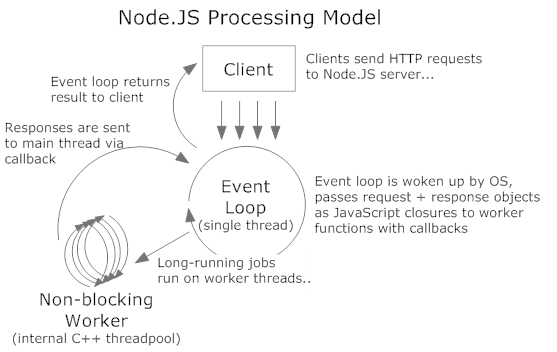
\includegraphics[width=12cm]{image.png}\]

\[\text{Model przetwarzania Node.js}\]

    \hypertarget{rozwiux105zania}{%
\section{Rozwiązania}\label{rozwiux105zania}}

    \hypertarget{node1a.js}{%
\subsection{\texorpdfstring{\texttt{node1a.js}}{node1a.js}}\label{node1a.js}}

Zgodnie z poleceniem, została utworzona funkcja \texttt{loop}, ktora
powoduje wykonanie sekwencji zadań \texttt{m} razy.

Cały kod źródłowy:

\begin{Shaded}
\begin{Highlighting}[]
\KeywordTok{function} \FunctionTok{printAsync}\NormalTok{(s}\OperatorTok{,}\NormalTok{ callback) \{}
    \KeywordTok{var}\NormalTok{ delay }\OperatorTok{=} \BuiltInTok{Math}\OperatorTok{.}\FunctionTok{floor}\NormalTok{((}\BuiltInTok{Math}\OperatorTok{.}\FunctionTok{random}\NormalTok{() }\OperatorTok{*} \DecValTok{1000}\NormalTok{) }\OperatorTok{+} \DecValTok{500}\NormalTok{)}\OperatorTok{;}

    \PreprocessorTok{setTimeout}\NormalTok{(() }\KeywordTok{=\textgreater{}}\NormalTok{ \{}
        \BuiltInTok{console}\OperatorTok{.}\FunctionTok{log}\NormalTok{(s)}\OperatorTok{;}

        \ControlFlowTok{if}\NormalTok{ (callback) \{}
            \FunctionTok{callback}\NormalTok{()}\OperatorTok{;}
\NormalTok{        \}}
\NormalTok{    \}}\OperatorTok{,}\NormalTok{ delay)}\OperatorTok{;}
\NormalTok{\}}

\KeywordTok{function} \FunctionTok{loop}\NormalTok{(n) \{}
    \ControlFlowTok{if}\NormalTok{ (n }\OperatorTok{==} \DecValTok{0}\NormalTok{) \{}
        \BuiltInTok{console}\OperatorTok{.}\FunctionTok{log}\NormalTok{(}\StringTok{\textquotesingle{}done!\textquotesingle{}}\NormalTok{)}\OperatorTok{;}
        \ControlFlowTok{return}\OperatorTok{;}
\NormalTok{    \}}

    \FunctionTok{printAsync}\NormalTok{(}\DecValTok{1}\OperatorTok{,}\NormalTok{ () }\KeywordTok{=\textgreater{}}\NormalTok{ \{}
        \FunctionTok{printAsync}\NormalTok{(}\DecValTok{2}\OperatorTok{,}\NormalTok{ () }\KeywordTok{=\textgreater{}}\NormalTok{ \{}
            \FunctionTok{printAsync}\NormalTok{(}\DecValTok{3}\OperatorTok{,}\NormalTok{ () }\KeywordTok{=\textgreater{}}\NormalTok{ \{}
                \FunctionTok{loop}\NormalTok{(n }\OperatorTok{{-}} \DecValTok{1}\NormalTok{)}\OperatorTok{;}
\NormalTok{            \})}\OperatorTok{;}
\NormalTok{        \})}\OperatorTok{;}
\NormalTok{    \})}\OperatorTok{;}
\NormalTok{\}}

\FunctionTok{loop}\NormalTok{(}\DecValTok{3}\NormalTok{)}\OperatorTok{;}
\end{Highlighting}
\end{Shaded}

Jak widać z powyższej implementacji, została użyta rekursja z warunkiem
stopu \texttt{n\ ==\ 0}: po wypisaniu ostatniej liczby w iteracji
\texttt{n} funkcja \texttt{loop} zostanie wywołana z argumentem
\texttt{n\ -\ 1}.

    \hypertarget{node1b.js}{%
\subsection{\texorpdfstring{\texttt{node1b.js}}{node1b.js}}\label{node1b.js}}

Zgodnie z poleceniem, skorzystano z funkcji \texttt{waterfall}
biblioteki \texttt{async}.

    Z dokumentacji:

\begin{quote}
Runs the tasks array of functions in series, each passing their results
to the next in the array. However, if any of the tasks pass an error to
their own callback, the next function is not executed, and the main
callback is immediately called with the error.
\end{quote}

Co w skrócie oznacza, że jest to sposób na uporządkowanie wykonywania
funkcji, które zależą od wyników poprzednich funkcji, bez blokowania
głównego wątku.

    \[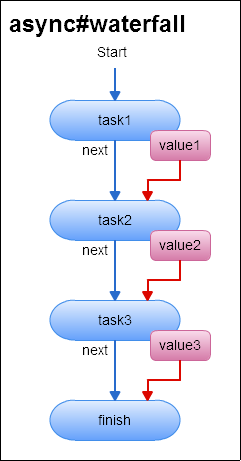
\includegraphics[height=8cm]{async_waterfall.png}\]

\[\text{Schemat działania funkcji \texttt{async\#waterfall}}\]

    Rozwiązanie wykorzystujące tylko już zdefiniowane funkcje, ale
niepoprawne z punktu widzenia dokumentacji:

\begin{Shaded}
\begin{Highlighting}[]
\KeywordTok{const} \KeywordTok{async} \OperatorTok{=} \PreprocessorTok{require}\NormalTok{(}\StringTok{\textquotesingle{}async\textquotesingle{}}\NormalTok{)}\OperatorTok{;}

\CommentTok{/**}
\CommentTok{ * }\AnnotationTok{@param}\CommentTok{ }\CommentVarTok{\{any\}}\CommentTok{ s }
\CommentTok{ * }\AnnotationTok{@param}\CommentTok{ }\CommentVarTok{\{}\CommentTok{() =\textgreater{} void\} callback }
\CommentTok{ */}
\KeywordTok{function} \FunctionTok{printAsync}\NormalTok{(s}\OperatorTok{,}\NormalTok{ callback) \{}
    \KeywordTok{let}\NormalTok{ delay }\OperatorTok{=} \BuiltInTok{Math}\OperatorTok{.}\FunctionTok{floor}\NormalTok{((}\BuiltInTok{Math}\OperatorTok{.}\FunctionTok{random}\NormalTok{() }\OperatorTok{*} \DecValTok{1000}\NormalTok{) }\OperatorTok{+} \DecValTok{500}\NormalTok{)}\OperatorTok{;}

    \PreprocessorTok{setTimeout}\NormalTok{(() }\KeywordTok{=\textgreater{}}\NormalTok{ \{}
        \BuiltInTok{console}\OperatorTok{.}\FunctionTok{log}\NormalTok{(s)}\OperatorTok{;}

        \ControlFlowTok{if}\NormalTok{ (callback) \{}
            \FunctionTok{callback}\NormalTok{()}\OperatorTok{;}
\NormalTok{        \}}
\NormalTok{    \}}\OperatorTok{,}\NormalTok{ delay)}\OperatorTok{;}
\NormalTok{\}}

\KeywordTok{function} \FunctionTok{task1}\NormalTok{(callback) \{}
    \FunctionTok{printAsync}\NormalTok{(}\StringTok{"1"}\OperatorTok{,}\NormalTok{ callback)}\OperatorTok{;}
\NormalTok{\}}

\KeywordTok{function} \FunctionTok{task2}\NormalTok{(callback) \{}
    \FunctionTok{printAsync}\NormalTok{(}\StringTok{"2"}\OperatorTok{,}\NormalTok{ callback)}\OperatorTok{;}
\NormalTok{\}}

\KeywordTok{function} \FunctionTok{task3}\NormalTok{(callback) \{}
    \FunctionTok{printAsync}\NormalTok{(}\StringTok{"3"}\OperatorTok{,}\NormalTok{ callback)}\OperatorTok{;}
\NormalTok{\}}

\KeywordTok{async}\OperatorTok{.}\FunctionTok{waterfall}\NormalTok{([}
\NormalTok{    task1}\OperatorTok{,}
\NormalTok{    task2}\OperatorTok{,}
\NormalTok{    task3}
\NormalTok{])}\OperatorTok{.}\FunctionTok{then}\NormalTok{((val) }\KeywordTok{=\textgreater{}}\NormalTok{ \{}
    \BuiltInTok{console}\OperatorTok{.}\FunctionTok{log}\NormalTok{(val)}\OperatorTok{;}
\NormalTok{\})}
\end{Highlighting}
\end{Shaded}

\emph{Wyniki zostaną omówione w odpowiednim rozdziale.}

\textbf{Rozwiązanie to nie jest zgodne z dokumentacją} ze względu na
sygnaturę funkcji \texttt{callback}:

\begin{quote}
An optional callback to run once all the functions have completed. This
will be passed the results of the last task's callback. \textbf{Invoked
with (err, {[}results{]})}.
\end{quote}

Oczekiwana sygnatura:

\begin{Shaded}
\begin{Highlighting}[]
\NormalTok{(e}\OperatorTok{:} \BuiltInTok{Error}\OperatorTok{,}\NormalTok{ [results]) }\KeywordTok{=\textgreater{}} \KeywordTok{void}
\end{Highlighting}
\end{Shaded}

Ale mamy:

\begin{Shaded}
\begin{Highlighting}[]
\NormalTok{() }\KeywordTok{=\textgreater{}} \KeywordTok{void}
\end{Highlighting}
\end{Shaded}

    \textbf{Rozwiązanie zgodne z dokumentacją:}

\begin{Shaded}
\begin{Highlighting}[]
\KeywordTok{const} \KeywordTok{async} \OperatorTok{=} \PreprocessorTok{require}\NormalTok{(}\StringTok{\textquotesingle{}async\textquotesingle{}}\NormalTok{)}\OperatorTok{;}

\CommentTok{/**}
\CommentTok{ * }\AnnotationTok{@param}\CommentTok{ }\CommentVarTok{\{any\}}\CommentTok{ s }
\CommentTok{ * }\AnnotationTok{@param}\CommentTok{ }\CommentVarTok{\{}\CommentTok{(e: Error, [results]) =\textgreater{} void\} callback }
\CommentTok{ */}
\KeywordTok{function} \FunctionTok{callAsync}\NormalTok{(s}\OperatorTok{,}\NormalTok{ callback) \{}
    \KeywordTok{var}\NormalTok{ delay }\OperatorTok{=} \BuiltInTok{Math}\OperatorTok{.}\FunctionTok{floor}\NormalTok{((}\BuiltInTok{Math}\OperatorTok{.}\FunctionTok{random}\NormalTok{() }\OperatorTok{*} \DecValTok{1000}\NormalTok{) }\OperatorTok{+} \DecValTok{500}\NormalTok{)}\OperatorTok{;}

    \PreprocessorTok{setTimeout}\NormalTok{(() }\KeywordTok{=\textgreater{}}\NormalTok{ \{}
        \BuiltInTok{console}\OperatorTok{.}\FunctionTok{log}\NormalTok{(}\StringTok{"Running"}\OperatorTok{,}\NormalTok{ s)}

        \ControlFlowTok{if}\NormalTok{ (callback) \{}
            \FunctionTok{callback}\NormalTok{(}\KeywordTok{null}\OperatorTok{,}\NormalTok{ s)}\OperatorTok{;}
\NormalTok{        \}}
\NormalTok{    \}}\OperatorTok{,}\NormalTok{ delay)}\OperatorTok{;}
\NormalTok{\}}

\CommentTok{// https://caolan.github.io/async/v3/docs.html\#waterfall}

\KeywordTok{async}\OperatorTok{.}\FunctionTok{waterfall}\NormalTok{([}
\NormalTok{    callback }\KeywordTok{=\textgreater{}}\NormalTok{ \{}
        \FunctionTok{callAsync}\NormalTok{(}\DecValTok{1}\OperatorTok{,}\NormalTok{ callback)}\OperatorTok{;}
\NormalTok{    \}}\OperatorTok{,}
\NormalTok{    (prev}\OperatorTok{,}\NormalTok{ callback) }\KeywordTok{=\textgreater{}}\NormalTok{ \{}
        \BuiltInTok{console}\OperatorTok{.}\FunctionTok{log}\NormalTok{(}\StringTok{"Task"}\OperatorTok{,}\NormalTok{ prev}\OperatorTok{,} \StringTok{"done"}\NormalTok{)}\OperatorTok{;}
        \FunctionTok{callAsync}\NormalTok{(}\DecValTok{2}\OperatorTok{,}\NormalTok{ callback)}
\NormalTok{    \}}\OperatorTok{,}
\NormalTok{    (prev}\OperatorTok{,}\NormalTok{ callback) }\KeywordTok{=\textgreater{}}\NormalTok{ \{}
        \BuiltInTok{console}\OperatorTok{.}\FunctionTok{log}\NormalTok{(}\StringTok{"Task"}\OperatorTok{,}\NormalTok{ prev}\OperatorTok{,} \StringTok{"done"}\NormalTok{)}\OperatorTok{;}
        \FunctionTok{callAsync}\NormalTok{(}\DecValTok{3}\OperatorTok{,}\NormalTok{ callback)}\OperatorTok{;}
\NormalTok{    \}}
\NormalTok{])}\OperatorTok{.}\FunctionTok{then}\NormalTok{(val }\KeywordTok{=\textgreater{}}\NormalTok{ \{}
    \BuiltInTok{console}\OperatorTok{.}\FunctionTok{log}\NormalTok{(}\StringTok{"Task"}\OperatorTok{,}\NormalTok{ val}\OperatorTok{,} \StringTok{"done"}\NormalTok{)}\OperatorTok{;}
    \BuiltInTok{console}\OperatorTok{.}\FunctionTok{log}\NormalTok{(}\StringTok{"Done"}\NormalTok{)}\OperatorTok{;}
\NormalTok{\})}
\end{Highlighting}
\end{Shaded}

\emph{Wyniki zostaną omówione w odpowiednim rozdziale.}

    \textbf{Cała implementacja} jest następująca:

\begin{Shaded}
\begin{Highlighting}[]
\KeywordTok{const} \KeywordTok{async} \OperatorTok{=} \PreprocessorTok{require}\NormalTok{(}\StringTok{\textquotesingle{}async\textquotesingle{}}\NormalTok{)}\OperatorTok{;}

\CommentTok{/**}
\CommentTok{ * }\AnnotationTok{@param}\CommentTok{ }\CommentVarTok{\{any\}}\CommentTok{ s }
\CommentTok{ * }\AnnotationTok{@param}\CommentTok{ }\CommentVarTok{\{}\CommentTok{() =\textgreater{} void\} callback }
\CommentTok{ */}
\KeywordTok{function} \FunctionTok{printAsync}\NormalTok{(s}\OperatorTok{,}\NormalTok{ callback) \{}
    \KeywordTok{let}\NormalTok{ delay }\OperatorTok{=} \BuiltInTok{Math}\OperatorTok{.}\FunctionTok{floor}\NormalTok{((}\BuiltInTok{Math}\OperatorTok{.}\FunctionTok{random}\NormalTok{() }\OperatorTok{*} \DecValTok{1000}\NormalTok{) }\OperatorTok{+} \DecValTok{500}\NormalTok{)}\OperatorTok{;}

    \PreprocessorTok{setTimeout}\NormalTok{(() }\KeywordTok{=\textgreater{}}\NormalTok{ \{}
        \BuiltInTok{console}\OperatorTok{.}\FunctionTok{log}\NormalTok{(s)}\OperatorTok{;}

        \ControlFlowTok{if}\NormalTok{ (callback) \{}
            \FunctionTok{callback}\NormalTok{()}\OperatorTok{;}
\NormalTok{        \}}
\NormalTok{    \}}\OperatorTok{,}\NormalTok{ delay)}\OperatorTok{;}
\NormalTok{\}}

\KeywordTok{function} \FunctionTok{execute}\NormalTok{(tasks) \{}

    \KeywordTok{function} \FunctionTok{iterate}\NormalTok{(index) \{}
        \CommentTok{// tasks are finished}
        \ControlFlowTok{if}\NormalTok{ (index }\OperatorTok{===}\NormalTok{ tasks}\OperatorTok{.}\AttributeTok{length}\NormalTok{) \{}
            \ControlFlowTok{return}\OperatorTok{;}
\NormalTok{        \}}

        \CommentTok{// set the current task}
        \KeywordTok{const}\NormalTok{ task }\OperatorTok{=}\NormalTok{ tasks[index]}\OperatorTok{;}

        \CommentTok{/* executes the current task passing the \textquotesingle{}iterate\textquotesingle{} function as a}
\CommentTok{         * callback, it will be called by the task itself */}
        \FunctionTok{task}\NormalTok{(() }\KeywordTok{=\textgreater{}} \FunctionTok{iterate}\NormalTok{(index }\OperatorTok{+} \DecValTok{1}\NormalTok{))}\OperatorTok{;}
\NormalTok{    \}}

    \ControlFlowTok{return} \FunctionTok{iterate}\NormalTok{(}\DecValTok{0}\NormalTok{)}\OperatorTok{;}
\NormalTok{\}}

\KeywordTok{function} \FunctionTok{task1}\NormalTok{(callback) \{}
    \FunctionTok{printAsync}\NormalTok{(}\StringTok{"1"}\OperatorTok{,}\NormalTok{ callback)}\OperatorTok{;}
\NormalTok{\}}

\KeywordTok{function} \FunctionTok{task2}\NormalTok{(callback) \{}
    \FunctionTok{printAsync}\NormalTok{(}\StringTok{"2"}\OperatorTok{,}\NormalTok{ callback)}\OperatorTok{;}
\NormalTok{\}}

\KeywordTok{function} \FunctionTok{task3}\NormalTok{(callback) \{}
    \FunctionTok{printAsync}\NormalTok{(}\StringTok{"3"}\OperatorTok{,}\NormalTok{ callback)}\OperatorTok{;}
\NormalTok{\}}

\CommentTok{/**}
\CommentTok{ * }\AnnotationTok{@param}\CommentTok{ }\CommentVarTok{\{any\}}\CommentTok{ s }
\CommentTok{ * }\AnnotationTok{@param}\CommentTok{ }\CommentVarTok{\{}\CommentTok{(e: Error, [results]) =\textgreater{} void\} callback }
\CommentTok{ */}
\KeywordTok{function} \FunctionTok{callAsync}\NormalTok{(s}\OperatorTok{,}\NormalTok{ callback) \{}
    \KeywordTok{var}\NormalTok{ delay }\OperatorTok{=} \BuiltInTok{Math}\OperatorTok{.}\FunctionTok{floor}\NormalTok{((}\BuiltInTok{Math}\OperatorTok{.}\FunctionTok{random}\NormalTok{() }\OperatorTok{*} \DecValTok{1000}\NormalTok{) }\OperatorTok{+} \DecValTok{500}\NormalTok{)}\OperatorTok{;}

    \PreprocessorTok{setTimeout}\NormalTok{(() }\KeywordTok{=\textgreater{}}\NormalTok{ \{}
        \BuiltInTok{console}\OperatorTok{.}\FunctionTok{log}\NormalTok{(}\StringTok{"Running"}\OperatorTok{,}\NormalTok{ s)}

        \ControlFlowTok{if}\NormalTok{ (callback) \{}
            \FunctionTok{callback}\NormalTok{(}\KeywordTok{null}\OperatorTok{,}\NormalTok{ s)}\OperatorTok{;}
\NormalTok{        \}}
\NormalTok{    \}}\OperatorTok{,}\NormalTok{ delay)}\OperatorTok{;}
\NormalTok{\}}

\KeywordTok{async} \KeywordTok{function} \FunctionTok{main}\NormalTok{() \{}
    \BuiltInTok{console}\OperatorTok{.}\FunctionTok{log}\NormalTok{(}\StringTok{"waterfall naive"}\NormalTok{)}

    \ControlFlowTok{await} \KeywordTok{async}\OperatorTok{.}\FunctionTok{waterfall}\NormalTok{([}
\NormalTok{        task1}\OperatorTok{,}
\NormalTok{        task2}\OperatorTok{,}
\NormalTok{        task3}
\NormalTok{    ])}\OperatorTok{.}\FunctionTok{then}\NormalTok{((val) }\KeywordTok{=\textgreater{}}\NormalTok{ \{}
        \BuiltInTok{console}\OperatorTok{.}\FunctionTok{log}\NormalTok{(val)}\OperatorTok{;}
\NormalTok{    \})}

    \BuiltInTok{console}\OperatorTok{.}\FunctionTok{log}\NormalTok{(}\StringTok{"waterfall"}\NormalTok{)}

    \CommentTok{// https://caolan.github.io/async/v3/docs.html\#waterfall}

    \ControlFlowTok{await} \KeywordTok{async}\OperatorTok{.}\FunctionTok{waterfall}\NormalTok{([}
\NormalTok{        callback }\KeywordTok{=\textgreater{}}\NormalTok{ \{}
            \FunctionTok{callAsync}\NormalTok{(}\DecValTok{1}\OperatorTok{,}\NormalTok{ callback)}\OperatorTok{;}
\NormalTok{        \}}\OperatorTok{,}
\NormalTok{        (prev}\OperatorTok{,}\NormalTok{ callback) }\KeywordTok{=\textgreater{}}\NormalTok{ \{}
            \BuiltInTok{console}\OperatorTok{.}\FunctionTok{log}\NormalTok{(}\StringTok{"Task"}\OperatorTok{,}\NormalTok{ prev}\OperatorTok{,} \StringTok{"done"}\NormalTok{)}\OperatorTok{;}
            \FunctionTok{callAsync}\NormalTok{(}\DecValTok{2}\OperatorTok{,}\NormalTok{ callback)}
\NormalTok{        \}}\OperatorTok{,}
\NormalTok{        (prev}\OperatorTok{,}\NormalTok{ callback) }\KeywordTok{=\textgreater{}}\NormalTok{ \{}
            \BuiltInTok{console}\OperatorTok{.}\FunctionTok{log}\NormalTok{(}\StringTok{"Task"}\OperatorTok{,}\NormalTok{ prev}\OperatorTok{,} \StringTok{"done"}\NormalTok{)}\OperatorTok{;}
            \FunctionTok{callAsync}\NormalTok{(}\DecValTok{3}\OperatorTok{,}\NormalTok{ callback)}\OperatorTok{;}
\NormalTok{        \}}
\NormalTok{    ])}\OperatorTok{.}\FunctionTok{then}\NormalTok{(val }\KeywordTok{=\textgreater{}}\NormalTok{ \{}
        \BuiltInTok{console}\OperatorTok{.}\FunctionTok{log}\NormalTok{(}\StringTok{"Task"}\OperatorTok{,}\NormalTok{ val}\OperatorTok{,} \StringTok{"done"}\NormalTok{)}\OperatorTok{;}
        \BuiltInTok{console}\OperatorTok{.}\FunctionTok{log}\NormalTok{(}\StringTok{"Done"}\NormalTok{)}\OperatorTok{;}
\NormalTok{    \})}
\NormalTok{\}}

\CommentTok{// execute([task1, task2, task3]);}

\FunctionTok{main}\NormalTok{()}
\end{Highlighting}
\end{Shaded}

    \hypertarget{node1c.js}{%
\subsection{\texorpdfstring{\texttt{node1c.js}}{node1c.js}}\label{node1c.js}}

Zgodnie z poleceniem, została utworzona funkcja \texttt{loop}, ktora
powoduje wykonanie sekwencji zadań \texttt{m} razy. Analogicznie do
zadania \texttt{node1a.js}, została użyta rekursja z warunkiem stopu
\texttt{n\ ==\ 0}: po wypisaniu ostatniej liczby w iteracji \texttt{n}
funkcja \texttt{loop} zostanie wywołana z argumentem \texttt{n\ -\ 1}.

Cały kod źródłowy:

\begin{Shaded}
\begin{Highlighting}[]
\KeywordTok{function} \FunctionTok{printAsync}\NormalTok{(s}\OperatorTok{,}\NormalTok{ callback) \{}
    \KeywordTok{var}\NormalTok{ delay }\OperatorTok{=} \BuiltInTok{Math}\OperatorTok{.}\FunctionTok{floor}\NormalTok{((}\BuiltInTok{Math}\OperatorTok{.}\FunctionTok{random}\NormalTok{() }\OperatorTok{*} \DecValTok{1000}\NormalTok{) }\OperatorTok{+} \DecValTok{500}\NormalTok{)}\OperatorTok{;}

    \PreprocessorTok{setTimeout}\NormalTok{(() }\KeywordTok{=\textgreater{}}\NormalTok{ \{}
        \BuiltInTok{console}\OperatorTok{.}\FunctionTok{log}\NormalTok{(s)}\OperatorTok{;}

        \ControlFlowTok{if}\NormalTok{ (callback) \{}
            \FunctionTok{callback}\NormalTok{()}\OperatorTok{;}
\NormalTok{        \}}
\NormalTok{    \}}\OperatorTok{,}\NormalTok{ delay)}\OperatorTok{;}
\NormalTok{\}}

\KeywordTok{function} \FunctionTok{task}\NormalTok{(n) \{}
    \ControlFlowTok{return} \KeywordTok{new} \BuiltInTok{Promise}\NormalTok{((resolve}\OperatorTok{,}\NormalTok{ reject) }\KeywordTok{=\textgreater{}}\NormalTok{ \{}
        \FunctionTok{printAsync}\NormalTok{(n}\OperatorTok{,}\NormalTok{ () }\KeywordTok{=\textgreater{}}\NormalTok{ \{}
            \FunctionTok{resolve}\NormalTok{(n)}\OperatorTok{;}
\NormalTok{        \})}\OperatorTok{;}
\NormalTok{    \})}\OperatorTok{;}
\NormalTok{\}}


\CommentTok{// \textquotesingle{}then\textquotesingle{} returns a new Promise, therefore we can chain another \textquotesingle{}then\textquotesingle{}.}
\CommentTok{// In this case \textquotesingle{}task(x)\textquotesingle{} directly returns a Promise object, however}
\CommentTok{// \textquotesingle{}then\textquotesingle{} could also return a value in which case it would be wrapped}
\CommentTok{// in a Promise that would be automatically resolved with that value.}

\CommentTok{/*}
\CommentTok{** Zadanie:}
\CommentTok{** Napisz funkcje loop(m), ktora powoduje wykonanie powyzszej}
\CommentTok{** sekwencji zadan m razy.}
\CommentTok{**}
\CommentTok{*/}

\KeywordTok{function} \FunctionTok{loop}\NormalTok{(m) \{}
    \ControlFlowTok{if}\NormalTok{ (m }\OperatorTok{==} \DecValTok{0}\NormalTok{)}
        \ControlFlowTok{return}\OperatorTok{;}

    \FunctionTok{task}\NormalTok{(}\DecValTok{1}\NormalTok{)}\OperatorTok{.}\FunctionTok{then}\NormalTok{((n) }\KeywordTok{=\textgreater{}}\NormalTok{ \{}
        \BuiltInTok{console}\OperatorTok{.}\FunctionTok{log}\NormalTok{(}\StringTok{\textquotesingle{}task\textquotesingle{}}\OperatorTok{,}\NormalTok{ n}\OperatorTok{,} \StringTok{\textquotesingle{}done\textquotesingle{}}\NormalTok{)}\OperatorTok{;}
        \ControlFlowTok{return} \FunctionTok{task}\NormalTok{(}\DecValTok{2}\NormalTok{)}\OperatorTok{;}
\NormalTok{    \})}\OperatorTok{.}\FunctionTok{then}\NormalTok{((n) }\KeywordTok{=\textgreater{}}\NormalTok{ \{}
        \BuiltInTok{console}\OperatorTok{.}\FunctionTok{log}\NormalTok{(}\StringTok{\textquotesingle{}task\textquotesingle{}}\OperatorTok{,}\NormalTok{ n}\OperatorTok{,} \StringTok{\textquotesingle{}done\textquotesingle{}}\NormalTok{)}\OperatorTok{;}
        \ControlFlowTok{return} \FunctionTok{task}\NormalTok{(}\DecValTok{3}\NormalTok{)}\OperatorTok{;}
\NormalTok{    \})}\OperatorTok{.}\FunctionTok{then}\NormalTok{((n) }\KeywordTok{=\textgreater{}}\NormalTok{ \{}
        \BuiltInTok{console}\OperatorTok{.}\FunctionTok{log}\NormalTok{(}\StringTok{\textquotesingle{}task\textquotesingle{}}\OperatorTok{,}\NormalTok{ n}\OperatorTok{,} \StringTok{\textquotesingle{}done\textquotesingle{}}\NormalTok{)}\OperatorTok{;}
        \BuiltInTok{console}\OperatorTok{.}\FunctionTok{log}\NormalTok{(}\StringTok{\textquotesingle{}done!\textquotesingle{}}\NormalTok{)}\OperatorTok{;}
\NormalTok{    \})}\OperatorTok{.}\FunctionTok{then}\NormalTok{(() }\KeywordTok{=\textgreater{}}\NormalTok{ \{}
        \FunctionTok{loop}\NormalTok{(m }\OperatorTok{{-}} \DecValTok{1}\NormalTok{)}\OperatorTok{;}
\NormalTok{    \})}\OperatorTok{;}
\NormalTok{\}}

\FunctionTok{loop}\NormalTok{(}\DecValTok{4}\NormalTok{)}\OperatorTok{;}
\end{Highlighting}
\end{Shaded}

    \hypertarget{node2t.js}{%
\subsection{\texorpdfstring{\texttt{node2t.js}}{node2t.js}}\label{node2t.js}}

Zgodnie z instrukcjami, został napisany program obliczający liczbę linii
we wszystkich plikach tekstowych z zadanego drzewa katalogów. Do testów
wykorzystano zbiór danych \emph{Traceroute Data}, który musi zostać
umieszczony w tym samym katalogu co i plik \texttt{package.json} oraz
\texttt{node\_modules}, tzn. struktura powinna wyglądać w sposób
następujący:

\begin{verbatim}
tw-lab9
    hello_world.js
    node_modules
    package.json
    package-lock.json
    PAM08
    tasks
\end{verbatim}

To zadanie zostało zaimplementowane \textbf{na 2 różne sposoby}:

\begin{itemize}
\tightlist
\item
  z synchronicznym (jeden po drugim) przetwarzaniem plików
\item
  z asynchronicznym (jednoczesnym) przetwarzaniem plików
\end{itemize}

    Implementacja znajduje się w pliku \texttt{node2.js} i wygląda w sposób
następujący:

\begin{Shaded}
\begin{Highlighting}[]
\KeywordTok{const}\NormalTok{ fs }\OperatorTok{=} \PreprocessorTok{require}\NormalTok{(}\StringTok{"fs"}\NormalTok{)}\OperatorTok{;}

\NormalTok{module}\OperatorTok{.}\AttributeTok{exports} \OperatorTok{=}\NormalTok{ \{}
    \DataTypeTok{countSync}\OperatorTok{:}\NormalTok{ countSync}\OperatorTok{,}
    \DataTypeTok{countAsync}\OperatorTok{:}\NormalTok{ countAsync}
\NormalTok{\}}

\CommentTok{/**}
\CommentTok{ * }\AnnotationTok{@param}\CommentTok{ }\CommentVarTok{\{string\}}\CommentTok{ path }
\CommentTok{ * }\AnnotationTok{@param}\CommentTok{ }\CommentVarTok{\{}\CommentTok{(path: string, count: number) =\textgreater{} void | undefined\} callback }
\CommentTok{ * }\AnnotationTok{@returns}\CommentTok{ \{Promise}\KeywordTok{\textless{}void\textgreater{}}\CommentTok{\}}
\CommentTok{ */}
\KeywordTok{async} \KeywordTok{function} \FunctionTok{countSync}\NormalTok{(path}\OperatorTok{,}\NormalTok{ callback) \{}
    \ControlFlowTok{await} \FunctionTok{forEachFile}\NormalTok{(path}\OperatorTok{,} \KeywordTok{async}\NormalTok{ file }\KeywordTok{=\textgreater{}}\NormalTok{ \{}
        \KeywordTok{const}\NormalTok{ lines }\OperatorTok{=} \ControlFlowTok{await} \FunctionTok{countLines}\NormalTok{(file)}\OperatorTok{;}

        \ControlFlowTok{if}\NormalTok{ (callback) \{}
            \FunctionTok{callback}\NormalTok{(file}\OperatorTok{,}\NormalTok{ lines)}
\NormalTok{        \}}
\NormalTok{    \})}
\NormalTok{\}}

\CommentTok{/**}
\CommentTok{ * }\AnnotationTok{@param}\CommentTok{ }\CommentVarTok{\{string\}}\CommentTok{ path }
\CommentTok{ * }\AnnotationTok{@param}\CommentTok{ }\CommentVarTok{\{}\CommentTok{(path: string, count: number) =\textgreater{} void | undefined\} callback}
\CommentTok{ * }\AnnotationTok{@returns}\CommentTok{ \{Promise}\KeywordTok{\textless{}void\textgreater{}}\CommentTok{\} }
\CommentTok{ */}
\KeywordTok{async} \KeywordTok{function} \FunctionTok{countAsync}\NormalTok{(path}\OperatorTok{,}\NormalTok{ callback) \{}
    \ControlFlowTok{return} \KeywordTok{new} \BuiltInTok{Promise}\NormalTok{(}\KeywordTok{async}\NormalTok{ resolve }\KeywordTok{=\textgreater{}}\NormalTok{ \{}
        \KeywordTok{let}\NormalTok{ counter }\OperatorTok{=} \DecValTok{0}
        \KeywordTok{let}\NormalTok{ treeBuilt }\OperatorTok{=} \KeywordTok{false}

        \ControlFlowTok{await} \FunctionTok{forEachFile}\NormalTok{(path}\OperatorTok{,}\NormalTok{ file }\KeywordTok{=\textgreater{}}\NormalTok{ \{}
            \OperatorTok{++}\NormalTok{counter}

            \FunctionTok{countLines}\NormalTok{(file)}\OperatorTok{.}\FunctionTok{then}\NormalTok{(val }\KeywordTok{=\textgreater{}}\NormalTok{ \{}
                \OperatorTok{{-}{-}}\NormalTok{counter}

                \ControlFlowTok{if}\NormalTok{ (callback) \{}
                    \FunctionTok{callback}\NormalTok{(file}\OperatorTok{,}\NormalTok{ val)}
\NormalTok{                \}}

                \ControlFlowTok{if}\NormalTok{ (counter }\OperatorTok{==} \DecValTok{0} \OperatorTok{\&\&}\NormalTok{ treeBuilt) \{}
                    \FunctionTok{resolve}\NormalTok{()}
\NormalTok{                \}}
\NormalTok{            \})}
\NormalTok{        \})}

\NormalTok{        treeBuilt }\OperatorTok{=} \KeywordTok{true}
\NormalTok{    \})}
\NormalTok{\}}

\KeywordTok{async} \KeywordTok{function} \FunctionTok{forEachFile}\NormalTok{(dir}\OperatorTok{,}\NormalTok{ callback) \{}
    \ControlFlowTok{for}\NormalTok{ (}\KeywordTok{let}\NormalTok{ file }\KeywordTok{of}\NormalTok{ fs}\OperatorTok{.}\FunctionTok{readdirSync}\NormalTok{(dir)) \{}
\NormalTok{        file }\OperatorTok{=}\NormalTok{ dir }\OperatorTok{+} \StringTok{"/"} \OperatorTok{+}\NormalTok{ file}

        \ControlFlowTok{if}\NormalTok{ (fs}\OperatorTok{.}\FunctionTok{statSync}\NormalTok{(file)}\OperatorTok{.}\FunctionTok{isDirectory}\NormalTok{()) \{}
            \ControlFlowTok{await} \FunctionTok{forEachFile}\NormalTok{(file}\OperatorTok{,}\NormalTok{ callback)}
\NormalTok{        \} }\ControlFlowTok{else}\NormalTok{ \{}
            \ControlFlowTok{await} \FunctionTok{callback}\NormalTok{(file)}
\NormalTok{        \}}
\NormalTok{    \}}
\NormalTok{\}}

\KeywordTok{async} \KeywordTok{function} \FunctionTok{countLines}\NormalTok{(filename) \{}
    \ControlFlowTok{return} \KeywordTok{new} \BuiltInTok{Promise}\NormalTok{((resolve}\OperatorTok{,}\NormalTok{ reject) }\KeywordTok{=\textgreater{}}\NormalTok{ \{}
        \KeywordTok{let}\NormalTok{ count }\OperatorTok{=} \DecValTok{0}

\NormalTok{        fs}\OperatorTok{.}\FunctionTok{createReadStream}\NormalTok{(filename)}\OperatorTok{.}\FunctionTok{on}\NormalTok{(}\StringTok{\textquotesingle{}data\textquotesingle{}}\OperatorTok{,} \KeywordTok{function}\NormalTok{(chunk) \{}
\NormalTok{            count }\OperatorTok{+=}\NormalTok{ chunk}\OperatorTok{.}\FunctionTok{toString}\NormalTok{(}\StringTok{\textquotesingle{}utf8\textquotesingle{}}\NormalTok{)}
                \OperatorTok{.}\FunctionTok{split}\NormalTok{(}\SpecialStringTok{/}\SpecialCharTok{\textbackslash{}r\textbackslash{}n|[\textbackslash{}n\textbackslash{}r\textbackslash{}u0085\textbackslash{}u2028\textbackslash{}u2029]}\SpecialStringTok{/g}\NormalTok{)}
                \OperatorTok{.}\AttributeTok{length} \OperatorTok{{-}} \DecValTok{1}\OperatorTok{;}
\NormalTok{        \})}\OperatorTok{.}\FunctionTok{on}\NormalTok{(}\StringTok{\textquotesingle{}end\textquotesingle{}}\OperatorTok{,} \KeywordTok{function}\NormalTok{() \{}
            \FunctionTok{resolve}\NormalTok{(count)}
\NormalTok{        \})}\OperatorTok{.}\FunctionTok{on}\NormalTok{(}\StringTok{\textquotesingle{}error\textquotesingle{}}\OperatorTok{,} \KeywordTok{function}\NormalTok{ (err) \{}
            \FunctionTok{reject}\NormalTok{(err)}
\NormalTok{        \})}\OperatorTok{;}
\NormalTok{    \})}
\NormalTok{\}}
\end{Highlighting}
\end{Shaded}

    Opis poszczególnych funkcji:

\begin{itemize}
\tightlist
\item
  \texttt{countSync} oblicza liczbę linii w sposób synchroniczny, tzn.
  przetwarza pliki jeden po drugim
\item
  \texttt{countAsync} oblicza liczbę linii w sposób asynchroniczny, tzn.
  przetwarza kilka plików jednocześnie

  \begin{itemize}
  \tightlist
  \item
    W implementacji można by było skorzystać z \texttt{Promise.all}, ale
    to wymagałoby najpierw stworzenia tablicy wszystkich promise'ów, z
    czego postanowiono zrezygnować
  \end{itemize}
\item
  \texttt{forEachFile} wywołuje \texttt{callback} dla każdego
  rekursywnie znalezionego pliku
\item
  \texttt{countLines} oblicza liczę linii w podanym pliku
\end{itemize}

    Implementacja porównywania szybkości działania tych implementacji
(\texttt{countSync} i \texttt{countAsync}) znajduje się w pliku
\texttt{node2t.js} i wygląda następująco:

\begin{Shaded}
\begin{Highlighting}[]
\KeywordTok{const}\NormalTok{ \{ countSync}\OperatorTok{,}\NormalTok{ countAsync \} }\OperatorTok{=} \PreprocessorTok{require}\NormalTok{(}\StringTok{"./node2.js"}\NormalTok{)}

\KeywordTok{const}\NormalTok{ DATASET\_DIR }\OperatorTok{=} \StringTok{"PAM08"}

\CommentTok{/**}
\CommentTok{ * }
\CommentTok{ * }\AnnotationTok{@param}\CommentTok{ }\CommentVarTok{\{async}\CommentTok{ () =\textgreater{} void\} func }
\CommentTok{ * }\AnnotationTok{@param}\CommentTok{ }\CommentVarTok{\{number\}}\CommentTok{ n }
\CommentTok{ * }\AnnotationTok{@returns}\CommentTok{ \{Promise}\KeywordTok{\textless{}number\textgreater{}}\CommentTok{\}}
\CommentTok{ */}
\KeywordTok{async} \KeywordTok{function} \FunctionTok{benchmark}\NormalTok{(func}\OperatorTok{,}\NormalTok{ n) \{}
    \KeywordTok{let}\NormalTok{ time }\OperatorTok{=} \DecValTok{0}

    \ControlFlowTok{for}\NormalTok{ (}\KeywordTok{let}\NormalTok{ i }\OperatorTok{=} \DecValTok{0}\OperatorTok{;}\NormalTok{ i }\OperatorTok{\textless{}}\NormalTok{ n}\OperatorTok{;} \OperatorTok{++}\NormalTok{i) \{}
        \KeywordTok{const}\NormalTok{ startTime }\OperatorTok{=} \BuiltInTok{Date}\OperatorTok{.}\FunctionTok{now}\NormalTok{()}
        \ControlFlowTok{await} \FunctionTok{func}\NormalTok{()}
\NormalTok{        time }\OperatorTok{+=} \BuiltInTok{Date}\OperatorTok{.}\FunctionTok{now}\NormalTok{() }\OperatorTok{{-}}\NormalTok{ startTime}
\NormalTok{    \}}

    \ControlFlowTok{return}\NormalTok{ time }\OperatorTok{/}\NormalTok{ n}\OperatorTok{;}
\NormalTok{\}}

\KeywordTok{async} \KeywordTok{function} \FunctionTok{runBenchmark}\NormalTok{() \{}
    \BuiltInTok{console}\OperatorTok{.}\FunctionTok{log}\NormalTok{(}\StringTok{"Starting syncMeanTime benchmark"}\NormalTok{)}
    \KeywordTok{const}\NormalTok{ syncMeanTime }\OperatorTok{=} \ControlFlowTok{await} \FunctionTok{benchmark}\NormalTok{(() }\KeywordTok{=\textgreater{}} \FunctionTok{countSync}\NormalTok{(DATASET\_DIR)}\OperatorTok{,} \DecValTok{100}\NormalTok{)}
    \BuiltInTok{console}\OperatorTok{.}\FunctionTok{log}\NormalTok{(}\StringTok{"syncMeanTime"}\OperatorTok{,}\NormalTok{ syncMeanTime)}

    \BuiltInTok{console}\OperatorTok{.}\FunctionTok{log}\NormalTok{(}\StringTok{"Starting asyncMeanTime benchmark"}\NormalTok{)}
    \KeywordTok{const}\NormalTok{ asyncMeanTime }\OperatorTok{=} \ControlFlowTok{await} \FunctionTok{benchmark}\NormalTok{(() }\KeywordTok{=\textgreater{}} \FunctionTok{countAsync}\NormalTok{(DATASET\_DIR)}\OperatorTok{,} \DecValTok{100}\NormalTok{)}
    \BuiltInTok{console}\OperatorTok{.}\FunctionTok{log}\NormalTok{(}\StringTok{"asyncMeanTime"}\OperatorTok{,}\NormalTok{ asyncMeanTime)}
\NormalTok{\}}

\KeywordTok{async} \KeywordTok{function} \FunctionTok{runDemo}\NormalTok{() \{}
    \KeywordTok{let}\NormalTok{ syncLineCount }\OperatorTok{=} \DecValTok{0}
    \KeywordTok{let}\NormalTok{ asyncLineCount }\OperatorTok{=} \DecValTok{0}

    \BuiltInTok{console}\OperatorTok{.}\FunctionTok{log}\NormalTok{(}\StringTok{"Sync line counter"}\NormalTok{)}

    \ControlFlowTok{await} \FunctionTok{countSync}\NormalTok{(}\StringTok{"PAM08"}\OperatorTok{,}\NormalTok{ (filename}\OperatorTok{,}\NormalTok{ count) }\KeywordTok{=\textgreater{}}\NormalTok{ \{}
        \BuiltInTok{console}\OperatorTok{.}\FunctionTok{log}\NormalTok{(filename}\OperatorTok{,}\NormalTok{ count)}
\NormalTok{        syncLineCount }\OperatorTok{+=}\NormalTok{ count}
\NormalTok{    \})}

    \BuiltInTok{console}\OperatorTok{.}\FunctionTok{log}\NormalTok{(}\StringTok{"Async line counter"}\NormalTok{)}

    \ControlFlowTok{await} \FunctionTok{countAsync}\NormalTok{(}\StringTok{"PAM08"}\OperatorTok{,}\NormalTok{ (filename}\OperatorTok{,}\NormalTok{ count) }\KeywordTok{=\textgreater{}}\NormalTok{ \{}
        \BuiltInTok{console}\OperatorTok{.}\FunctionTok{log}\NormalTok{(filename}\OperatorTok{,}\NormalTok{ count)}
\NormalTok{        asyncLineCount }\OperatorTok{+=}\NormalTok{ count}
\NormalTok{    \})}

    \BuiltInTok{console}\OperatorTok{.}\FunctionTok{assert}\NormalTok{(syncLineCount }\OperatorTok{==}\NormalTok{ asyncLineCount)}

    \BuiltInTok{console}\OperatorTok{.}\FunctionTok{log}\NormalTok{(}\StringTok{"Total line count:"}\OperatorTok{,}\NormalTok{ syncLineCount)}
\NormalTok{\}}

\CommentTok{// runDemo()}
\FunctionTok{runBenchmark}\NormalTok{()}
\end{Highlighting}
\end{Shaded}

    Opis poszczególnych funkcji:

\begin{itemize}
\tightlist
\item
  \texttt{benchmark} mierzy średni czas wykonania funkcji \texttt{func}
  uruchamiając ją \texttt{n} razy
\item
  \texttt{runBenchmark} uruchamia pomiary szybkości działania w/w
  implementacji
\item
  \texttt{runDemo} wypisuje pliki wraz z liczbą linii
\end{itemize}

    \hypertarget{wyniki}{%
\section{Wyniki}\label{wyniki}}

W tym rozdziale zostały umieszczone wyniki poszczególnych programów.

Podczas testowania został użyty następujący sprzęt i oprogramowanie:

\begin{itemize}
\tightlist
\item
  16 × AMD Ryzen 7 4800H with Radeon Graphics
\item
  Fedora 38, Linux 6.5.12-200.fc38.x86\_64
\item
  Node.js v21.2.0, npm 10.2.3
\end{itemize}

    \begin{tcolorbox}[breakable, size=fbox, boxrule=1pt, pad at break*=1mm,colback=cellbackground, colframe=cellborder]
\prompt{In}{incolor}{2}{\boxspacing}
\begin{Verbatim}[commandchars=\\\{\}]
\PY{c+ch}{\PYZsh{}!/bin/bash}
\PY{n+nb}{export}\PY{+w}{ }\PY{n+nv}{PATH}\PY{o}{=}\PY{l+s+s2}{\PYZdq{}}\PY{l+s+s2}{/home/congard/Dev/node\PYZhy{}v21.2.0\PYZhy{}linux\PYZhy{}x64/bin:}\PY{n+nv}{\PYZdl{}PATH}\PY{l+s+s2}{\PYZdq{}}
\end{Verbatim}
\end{tcolorbox}

    \begin{tcolorbox}[breakable, size=fbox, boxrule=1pt, pad at break*=1mm,colback=cellbackground, colframe=cellborder]
\prompt{In}{incolor}{4}{\boxspacing}
\begin{Verbatim}[commandchars=\\\{\}]
\PY{c+ch}{\PYZsh{}!/bin/bash}
node\PY{+w}{ }\PYZhy{}\PYZhy{}version
npm\PY{+w}{ }\PYZhy{}\PYZhy{}version
\end{Verbatim}
\end{tcolorbox}

    \begin{Verbatim}[commandchars=\\\{\}]
v21.2.0
10.2.3
    \end{Verbatim}

    \begin{tcolorbox}[breakable, size=fbox, boxrule=1pt, pad at break*=1mm,colback=cellbackground, colframe=cellborder]
\prompt{In}{incolor}{7}{\boxspacing}
\begin{Verbatim}[commandchars=\\\{\}]
\PY{c+ch}{\PYZsh{}!/bin/bash}
\PY{n+nb}{cd}\PY{+w}{ }\PY{l+s+s2}{\PYZdq{}TW/labs/tw\PYZhy{}lab9\PYZdq{}}
\end{Verbatim}
\end{tcolorbox}

    \hypertarget{node1.js}{%
\subsection{\texorpdfstring{\texttt{node1.js}}{node1.js}}\label{node1.js}}

    \begin{tcolorbox}[breakable, size=fbox, boxrule=1pt, pad at break*=1mm,colback=cellbackground, colframe=cellborder]
\prompt{In}{incolor}{9}{\boxspacing}
\begin{Verbatim}[commandchars=\\\{\}]
\PY{c+ch}{\PYZsh{}!/bin/bash}
\PY{k}{for}\PY{o}{(}\PY{o}{(}\PY{n+nv}{i}\PY{o}{=}\PY{l+m}{0}\PY{p}{;}i\PYZlt{}\PY{l+m}{3}\PY{p}{;}i++\PY{o}{)}\PY{o}{)}\PY{p}{;}
\PY{k}{do}
\PY{+w}{    }npm\PY{+w}{ }run\PY{+w}{ }node1
\PY{k}{done}
\end{Verbatim}
\end{tcolorbox}

    \begin{Verbatim}[commandchars=\\\{\}]

> tw-lab9@0.0.0 node1
> node tasks/node1.js

done!
3
1
2

> tw-lab9@0.0.0 node1
> node tasks/node1.js

done!
1
3
2

> tw-lab9@0.0.0 node1
> node tasks/node1.js

done!
2
3
1
    \end{Verbatim}

    Jak widać, na wejściu otrzymaliśmy liczby wypisane za każdym
uruchomieniem w różnej kolejności. To wynika z tego, że wypisywaliśmy je
asynchronicznie najpierw czekając przez wylosowany okres czasu.

    \hypertarget{node1a.js}{%
\subsection{\texorpdfstring{\texttt{node1a.js}}{node1a.js}}\label{node1a.js}}

    \begin{tcolorbox}[breakable, size=fbox, boxrule=1pt, pad at break*=1mm,colback=cellbackground, colframe=cellborder]
\prompt{In}{incolor}{10}{\boxspacing}
\begin{Verbatim}[commandchars=\\\{\}]
\PY{c+ch}{\PYZsh{}!/bin/bash}
npm\PY{+w}{ }run\PY{+w}{ }node1a
\end{Verbatim}
\end{tcolorbox}

    \begin{Verbatim}[commandchars=\\\{\}]

> tw-lab9@0.0.0 node1a
> node tasks/node1a.js

\textcolor{ansi-yellow}{1}
\textcolor{ansi-yellow}{2}
\textcolor{ansi-yellow}{3}
\textcolor{ansi-yellow}{1}
\textcolor{ansi-yellow}{2}
\textcolor{ansi-yellow}{3}
\textcolor{ansi-yellow}{1}
\textcolor{ansi-yellow}{2}
\textcolor{ansi-yellow}{3}
done!
    \end{Verbatim}

    Tym razem widać, że wszystkie liczby zostały wypisane w poprawnej
kolejności 3 razy, a więc funkcja \texttt{loop} działa poprawnie.

    \hypertarget{node1b.js}{%
\subsection{\texorpdfstring{\texttt{node1b.js}}{node1b.js}}\label{node1b.js}}

    \begin{tcolorbox}[breakable, size=fbox, boxrule=1pt, pad at break*=1mm,colback=cellbackground, colframe=cellborder]
\prompt{In}{incolor}{11}{\boxspacing}
\begin{Verbatim}[commandchars=\\\{\}]
\PY{c+ch}{\PYZsh{}!/bin/bash}
npm\PY{+w}{ }run\PY{+w}{ }node1b
\end{Verbatim}
\end{tcolorbox}

    \begin{Verbatim}[commandchars=\\\{\}]

> tw-lab9@0.0.0 node1b
> node tasks/node1b.js

waterfall naive
1
2
3
\textcolor{ansi-black-intense}{undefined}
waterfall
Running \textcolor{ansi-yellow}{1}
Task \textcolor{ansi-yellow}{1} done
Running \textcolor{ansi-yellow}{2}
Task \textcolor{ansi-yellow}{2} done
Running \textcolor{ansi-yellow}{3}
Task \textcolor{ansi-yellow}{3} done
Done
    \end{Verbatim}

    Widać, że w przypadku implementacji niezgodnej z dokumentacją na końcu
jako wynik funkcji \texttt{async\#waterfall} wypisuje się
\texttt{undefined}. W przypadku poprawnej implementacji, tego nie
obserwujemy - wszystko działa zgodnie z oczekiwaniami i dokumentacja.

    \hypertarget{node1c.js}{%
\subsection{\texorpdfstring{\texttt{node1c.js}}{node1c.js}}\label{node1c.js}}

    \begin{tcolorbox}[breakable, size=fbox, boxrule=1pt, pad at break*=1mm,colback=cellbackground, colframe=cellborder]
\prompt{In}{incolor}{12}{\boxspacing}
\begin{Verbatim}[commandchars=\\\{\}]
\PY{c+ch}{\PYZsh{}!/bin/bash}
npm\PY{+w}{ }run\PY{+w}{ }node1c
\end{Verbatim}
\end{tcolorbox}

    \begin{Verbatim}[commandchars=\\\{\}]

> tw-lab9@0.0.0 node1c
> node tasks/node1c.js

\textcolor{ansi-yellow}{1}
task \textcolor{ansi-yellow}{1} done
\textcolor{ansi-yellow}{2}
task \textcolor{ansi-yellow}{2} done
\textcolor{ansi-yellow}{3}
task \textcolor{ansi-yellow}{3} done
done!
\textcolor{ansi-yellow}{1}
task \textcolor{ansi-yellow}{1} done
\textcolor{ansi-yellow}{2}
task \textcolor{ansi-yellow}{2} done
\textcolor{ansi-yellow}{3}
task \textcolor{ansi-yellow}{3} done
done!
\textcolor{ansi-yellow}{1}
task \textcolor{ansi-yellow}{1} done
\textcolor{ansi-yellow}{2}
task \textcolor{ansi-yellow}{2} done
\textcolor{ansi-yellow}{3}
task \textcolor{ansi-yellow}{3} done
done!
\textcolor{ansi-yellow}{1}
task \textcolor{ansi-yellow}{1} done
\textcolor{ansi-yellow}{2}
task \textcolor{ansi-yellow}{2} done
\textcolor{ansi-yellow}{3}
task \textcolor{ansi-yellow}{3} done
done!
    \end{Verbatim}

    Wszystkie liczby zostały wypisane w poprawnej kolejności 4 razy, a więc
funkcja \texttt{loop} działa poprawnie.

    \hypertarget{node1d.js}{%
\subsection{\texorpdfstring{\texttt{node1d.js}}{node1d.js}}\label{node1d.js}}

    \begin{tcolorbox}[breakable, size=fbox, boxrule=1pt, pad at break*=1mm,colback=cellbackground, colframe=cellborder]
\prompt{In}{incolor}{13}{\boxspacing}
\begin{Verbatim}[commandchars=\\\{\}]
\PY{c+ch}{\PYZsh{}!/bin/bash}
npm\PY{+w}{ }run\PY{+w}{ }node1d
\end{Verbatim}
\end{tcolorbox}

    \begin{Verbatim}[commandchars=\\\{\}]

> tw-lab9@0.0.0 node1d
> node tasks/node1d.js

\textcolor{ansi-yellow}{1}
\textcolor{ansi-yellow}{2}
\textcolor{ansi-yellow}{3}
\textcolor{ansi-yellow}{1}
\textcolor{ansi-yellow}{2}
\textcolor{ansi-yellow}{3}
\textcolor{ansi-yellow}{1}
\textcolor{ansi-yellow}{2}
\textcolor{ansi-yellow}{3}
\textcolor{ansi-yellow}{1}
\textcolor{ansi-yellow}{2}
\textcolor{ansi-yellow}{3}
    \end{Verbatim}

    Wszystkie liczby zostały wypisane w poprawnej kolejności 4 razy, a więc
funkcja \texttt{loop} działa poprawnie.

    \hypertarget{node2t.js}{%
\subsection{\texorpdfstring{\texttt{node2t.js}}{node2t.js}}\label{node2t.js}}

    \begin{tcolorbox}[breakable, size=fbox, boxrule=1pt, pad at break*=1mm,colback=cellbackground, colframe=cellborder]
\prompt{In}{incolor}{14}{\boxspacing}
\begin{Verbatim}[commandchars=\\\{\}]
\PY{c+ch}{\PYZsh{}!/bin/bash}
npm\PY{+w}{ }run\PY{+w}{ }node2t
\end{Verbatim}
\end{tcolorbox}

    \begin{Verbatim}[commandchars=\\\{\}]

> tw-lab9@0.0.0 node2t
> node tasks/node2t.js

Starting syncMeanTime benchmark
syncMeanTime \textcolor{ansi-yellow}{301.22}
Starting asyncMeanTime benchmark
asyncMeanTime \textcolor{ansi-yellow}{128.19}
    \end{Verbatim}

    Z otrzymanych pomiarów wynika, że asynchroniczne przetwarzanie plików
jest ponad 2 razy szybsze w porównaniu z synchronicznym.

    \hypertarget{wnioski}{%
\section{Wnioski}\label{wnioski}}

\begin{itemize}
\item
  \textbf{Node.js jest środowiskiem uruchomieniowym} JavaScript, które
  umożliwia tworzenie aplikacji w tym języku działających poza
  przeglądarką;
\item
  \textbf{Node.js wykorzystuje silnik JavaScript V8}, który jest szybki
  i optymalizowany dla nowoczesnych standardów webowych;
\item
  \textbf{Node.js obsługuje wiele współbieżnych żądań} przy użyciu
  pojedynczego wątku i pętli zdarzeń, która deleguje zadania
  asynchroniczne do puli wątków;
\item
  \textbf{Node.js jest lekki, wydajny i skalowalny}, ponieważ nie
  blokuje głównego wątku i reaguje na zdarzenia, a nie na żądania;
\item
  \textbf{\texttt{await}/\texttt{async}}: jest to sposób na pracę z
  obietnicami (promises) w asynchronicznych funkcjach. Jest to tzw.
  syntactic sugar, czyli uproszczenie składni, które sprawia, że kod z
  obietnicami jest łatwiejszy do czytania i pisania. Dzięki temu kod
  asynchroniczny wygląda bardziej jak synchroniczny/proceduralny.
  Funkcje \texttt{async} zawsze zwracają \texttt{Promise}, nawet jeśli
  operacja, którą wykonują, jest synchroniczna;
\item
  \textbf{\texttt{Promise}}: jest to obiekt reprezentujący końcowy wynik
  operacji asynchronicznej. Obietnica może znajdować się \emph{w jednym
  z trzech stanów}: oczekującym (pending), spełnionym (fulfilled) lub
  odrzuconym (rejected). Główną zaletą \texttt{Promise} jest unikanie
  tzw. ``callback hell'', czyli zagnieżdżania wielu wywołań zwrotnych
  (callbacks), co może prowadzić do nieczytelnego kodu;
\item
  \textbf{Metoda \texttt{then}} jest używana do zarejestrowania
  callbacków, które będą wywoływane, gdy \texttt{Promise} zostanie
  spełniony lub odrzucony. Pierwszy argument to funkcja, która zostanie
  wywołana, gdy \texttt{Promise} zostanie spełniony (\texttt{resolve}),
  a drugi argument to funkcja, która zostanie wywołana, gdy
  \texttt{Promise} zostanie odrzucony (\texttt{reject});
\item
  \textbf{\texttt{async.waterfall}}: jest to funkcja z biblioteki
  \emph{\texttt{async.js}}, która pozwala na wykonanie serii
  asynchronicznych funkcji jeden po drugim. Każda kolejna funkcja
  otrzymuje wyniki poprzedniej funkcji. Jeśli któraś z funkcji przekaże
  błąd do swojego callbacku, nie zostaną wykonane żadne kolejne funkcje,
  a główny callback zostanie natychmiast wywołany z błędem;
\item
  Asynchroniczne (jednoczesne) przetwarzanie plików okazało się ponad 2
  razy szybsze w porównaniu z synchronicznym (jeden po drugim);
\end{itemize}

    \hypertarget{bibliografia}{%
\section{Bibliografia}\label{bibliografia}}

\begin{enumerate}
\def\labelenumi{\arabic{enumi}.}
\item
  Materiały do laboratorium, dr inż. Włodzimierz Funika:\\
  \url{https://home.agh.edu.pl/~funika/tw/lab-js/}
\item
  Zbiór danych \emph{Traceroute Data}:\\
  \url{http://home.agh.edu.pl/~funika/tw/lab-js/pam08.zip}
\item
  Node.js, Wikipedia:\\
  \url{https://en.wikipedia.org/wiki/Node.js}
\item
  Exploring Async.js -- async.waterfall and async.series, Pentacode:\\
  \url{https://www.penta-code.com/02-exploring-async-js-async-waterfall-and-async-series/}
\item
  \texttt{async}, Async Docs:\\
  \url{https://caolan.github.io/async/v3/docs.html}
\item
  \texttt{fs}, Node.js v21 Docs:\\
  \url{https://nodejs.org/docs/latest-v21.x/api/fs.html}
\item
  How do you get a list of the names of all files present in a directory
  in Node.js?, Stackoverflow Question:\\
  \url{https://stackoverflow.com/q/2727167}
\item
  Coordinating parallel execution in node.js, Stackoverflow Question:\\
  \url{https://stackoverflow.com/q/4631774}
\item
  \texttt{Promise.all}, MDN Web Docs:\\
  \url{https://developer.mozilla.org/en-US/docs/Web/JavaScript/Reference/Global_Objects/Promise/all}
\item
  Difference between promise and async await in Node.js,
  GeeksForGeeks:\\
  \url{https://www.geeksforgeeks.org/difference-between-promise-and-async-await-in-node-js/}
\item
  async/await vs.~Promises - Which should I use?, Delving Developer:\\
  \url{https://delvingdeveloper.com/posts/async-await-vs-promises}
\item
  How to Use JavaScript Promises -- Callbacks, Async/Await, and Promise
  Methods Explained, Yogesh Chavan, freeCodeCamp:\\
  \url{https://www.freecodecamp.org/news/javascript-promises-async-await-and-promise-methods/}
\end{enumerate}


    % Add a bibliography block to the postdoc
    
    
    
\end{document}
